
\documentclass{article}

\usepackage[margin=1.33in]{geometry}
\usepackage{p200}
\usepackage[colorlinks=true,linkcolor=blue]{hyperref}

\hypersetup{pdftitle = {Physics 203 } }
\hypersetup{pdfauthor = {}, pdfsubject = {Physics} }

\pagestyle{plain}

\begin{document}

\begin{center}
{\LARGE Physics 203 }
\vskip 0.25cm
{\large The microscopic source of force}

\vskip 0.25cm
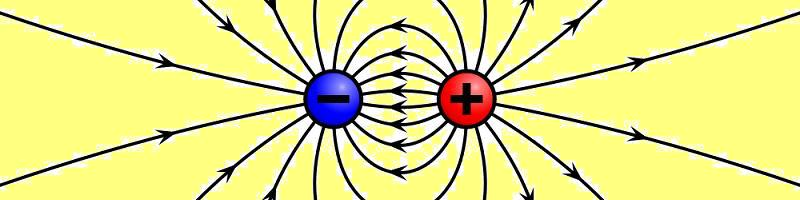
\includegraphics[width=\textwidth]{C:/"Program Files"/my/github/spot/content/banners/203.jpg}

\vskip 0.25cm
{\large Summer 2013}
\end{center}

\begin{center}
\renewcommand{\arraystretch}{1.5}
\renewcommand{\tabcolsep}{0.2cm}
\begin{tabular}{ll} 
\hline
Instructor & David J. Ulrich \\ 




\hline
\end{tabular}
\end{center}

\section{Course Overview}

This class rocks!

\clearpage



\section{Class Schedule}

This following schedule should be considered tentative. In particular, based on class progress, we may slow down or speed up the lecture schedule.

\begin{center}

\renewcommand{\arraystretch}{1.5}
\renewcommand{\tabcolsep}{0.2cm}

\begin{tabular}{@{}cccp{16mm}p{64mm}@{}}
%\begin{tabular}{cccll}
\hline
\textbf{Wk} &
\textbf{Day} &
\textbf{Date} &
\textbf{Type} &
\textbf{Title} &
\hline

1 &
Mon &
Jun 24 &
Lecture 1 &
Electric Field and Potential \\

1 &
Wed &
Jun 26 &
Lab 1 &
Projectiles and Free-Fall \\

\hline
\end{tabular}

\end{center}



\end{document}